% add. options: [seceqn,secthm,crcready,onecolumn]
\documentclass[jnr]{iosart2x}

%\usepackage{dcolumn}
%\usepackage{endnotes}

%%%%%%%%%%% Put your definitions here

\usepackage{listings}
\usepackage{rotating}

%%%%%%%%%%% End of definitions

\pubyear{0000}
\volume{0}
\firstpage{1}
\lastpage{1}

\begin{document}

\begin{frontmatter}

%\pretitle{}
\title{Guidelines for collaborative development of sustainable data treatment software}
\runningtitle{Guidelines for collaborative development of sustainable data treatment software}
%\subtitle{}

% Two or more authors:
\author[A]{\inits{D.}\fnms{Daniel} \snm{Nixon}\ead[label=e1]{daniel.nixon@stfc.ac.uk}%
\thanks{Corresponding author. \printead{e1}.}},
\author[A]{\inits{A.}\fnms{Anders} \snm{Markvardsen}\ead[label=e3]{anders.markvardsen@stfc.ac.uk}},
\author[C]{\inits{A.}\fnms{Anders} \snm{Kaestner}\ead[label=e5]{anders.kaestner@psi.ch}},
\author[D]{\inits{J.}\fnms{Joachim} \snm{Wuttke}\ead[label=e6]{j.wuttke@fz-juelich.de}},
\author[A]{\inits{S.}\fnms{Stephen} \snm{Cottrell}\ead[label=e7]{stephen.cottrell@stfc.ac.uk}},
\author[E]{\inits{M.}\fnms{Miguel} \snm{Gonzalez}\ead[label=e8]{gonzalezm@ill.fr}},
\author[A]{\inits{A.}\fnms{Anthony} \snm{Lim}\ead[label=e2]{anthony.lim@stfc.ac.uk}},
and
\author[B]{\inits{T.}\fnms{Thomas} \snm{Holm Rod}\ead[label=e4]{Thomas.HolmRod@esss.se}}

\runningauthor{D. Nixon et al.}
\address[A]{\orgname{Science and Technology Facilities Council},\cny{United Kingdom}\printead[presep={\\}]{e1,e2,e3,e7}}
\address[B]{\orgname{European Spallation Source},\cny{Sweden}\printead[presep={\\}]{e4}}
\address[C]{\orgname{Paul Scherrer Institute},\cny{Switzerland}\printead[presep={\\}]{e5}}
\address[D]{\orgname{Forschungszentrum Jülich},\cny{Germany}\printead[presep={\\}]{e6}}
\address[E]{\orgname{Institut Laue-Langevin},\cny{France}\printead[presep={\\}]{e8}}

\begin{abstract}
Scientific software is an essential part of the modern researcher's tool kit, due to large data sets and complex analysis techniques.
As a result the software is often expensive to develop.
Therefore, its imperative to ensure that the software will continue to be developed in the future, even if the current work force leaves the project.
Some of the requirements for sustainable software are for the code base to have a consistent quality and good documentation, to prevent a loss of knowledge.
This paper presents two sets of guidelines, a generic set that could be applied to a broad range of communities.
The second set of guidelines are specific to the neutron and muon data treatment communities and were developed as part of Science and Innovation with Neutrons in Europe in 2020 (SINE2020).

These specific guidelines were designed to allow the harmonization of software development.
Software outside of the neutron and muon data treatment communities can use the specific guidelines (TODO: section ref) as inspiration of how to apply the generic guidelines presented in this paper.
\end{abstract}

\begin{keyword}
\kwd{TODO}
\end{keyword}

\end{frontmatter}

%%%%%%%%%%% The article body starts:

\section{Introduction}
\label{Introduction}

It has become vital for modern neutron and muon sources to ensure that adequate user software is in existence not only for data acquisition but also for data treatment in order to ensure that the sources produce science rather than just data
The reason for this is at least two-fold 1) the demography of the users is changing from scientists building a career in neutron scattering or muon spectroscopy to scientists that consider neutron scattering and muon spectroscopy as tools among a broader set of tools and are thus not sufficient knowledgeable or skilled about the deeper details behind data treatment for neutron scattering or muon spectroscopy
Moreover, the users may simply not have the skills in how to analyse their data based on programs like MatLab, IDL, Python, or similar. 2) The advances in technology are leading to vast amounts of data that cannot be analysed by hand
For example, some instruments at the
European Spallation Source (ESS) are estimated to have data rates beyond [](TODO: Tobias’ paper) and at modern photon sources the situation is even more severe
This can be compared to the data rates from ten years ago, where ...(TODO: Historic example).
The growing complexity of both data reduction and analysis, means that the development of scientific software requires increasingly more resource.
The consequence of these aspects is that users inherently will depend on software developed by other developers typically at the facilities or in the user community, which in turn add significant requirements to quality, trustability, reliability and usability compared to when a developer develops software for herself or her colleague sitting next door

The lack of guidelines can lead to the code being difficult to read, because the style will change depending on who wrote it.
In the worst cases this can lead to people believing that the code is incorrect, when it is correct, hence leading to wasted effort.
The other potential pitfalls with this isolated approach of software development is that bugs are less likely to be found, due to less users.
Also the software may become too cumbersome to develop leading to the project having to start from scratch.
Inherently, these factors make it more difficult to share and for other research groups or research infrastructures to adapt the software for their own purpose.
Guidelines for software development ensure that the code is of a high quality and that the project progress effectively.
A good set of guidelines will help the software be:
\begin{itemize}
  \item reliable
  \item inter-operable
  \item extensible
  \item intuitive
  \item maintainable
\end{itemize}

Therefore, it will be easier to continue growing the code base to include new scientific analysis and techniques.
It would also reduce the effort required to adapt the software for use at other facilities.

Generic software development guidelines (TODO: cite) have been common practice for many years.
Specific software guidelines have been created for several scientific communities (TODO: cites).

The specific guidelines (TODO ref SINE2020 secion) presented in this paper were developed as part of SINE2020.
The software developed as part of SINE2020 had a broad range of team sizes.
From a couple of developers working very closely on a single piece of software to international collaborations.

Although the specific guidelines are aimed at the neutron and muon communities, the generic guidelines reflect what is common practice in software development.
Hence, when it is appropriate the idea of the guideline will be abstracted so that an alternative can be chosen in the future.
Abstracting guidelines in this manner allow then to remain relevant as technology evolves.
For instance, Python is today the de facto standard scripting language in scientific computing even though the first scientific python conference to the best of our knowledge was held as late as in 2002 with the scipy conference in Pasadena [] (TODO: ref and write something better.)

\section{Business as Usual}
\label{Business as Usual}

This section describes the day-to-day work of the developers working on the software.
This section will discuss the typical tasks performed by developers, such as development methodologies, code review and coding standards.
Another important part of the developers job is to provide documentation for users and other developers.
This reduces the risk of having single points of failure, because another developer can read the documentation and then continue the work.
Most of these choices will be made at the start of the project and ideally last its duration, however these can be updated to accommodate new tools and standards.

\subsection{Development methodology}
\label{Development methodology}

Development methodology is the set of rules that determine how requirements are gathered, converted into developer tasks and how the software is delivered to the user.

The two extremes of software development methodologies are called "agile" and "waterfall".
In the following we will discuss these to extremes, however in reality there is a scale and a mixture of these two extremes can be used.

For scientific software agile, or some variant of that, is the most common methodology.
The general principle of the agile methodology are short development "sprints" in which small, incremental additions are made to the overall software.
The requirements are reviewed and adjusted accordingly for each sprint.
This allows requirements to change quickly, reducing the delay in obtaining feedback from users and developers to be more responsive to the users' needs.

If there are set of fixed non-negotiable requirements then the waterfall methodology is better.
For the waterfall methodology each task is planned in advance and carried out in a predetermined order.
This ensures that the requirements are met and at key milestones.
However, the waterfall method lacks flexibility, making it difficult to respond to a change in requirements.
Projects that are better suited to the waterfall methodology are those where delivering an intermediate product is not viable.
For example, a library to perform Fourier transformations is not useful unless fully implemented whereas a graphical data processing toolkit could be useful mid way through development.

In reality a mixture of the two is usually implemented.
For example, a graphical user interface (GUI) that has a set of requirements (e.g. load data, do a fit to the data, output results).
To make sure that the GUI meets the requirements a waterfall approach could be used.
However, within that approach a more agile like methodology could be used.
The first two sprints could focus on loading and fitting to data.
The third sprint could then focus on making sure they interact with each other correctly.

\subsection{Coding standards}
\label{Coding standards}

Code should be of a high quality, the reason for this is two fold; code that conforms to accepted standards is more likely to be well formatted, readable and contain fewer bugs.
These factors combine to create a code base that is easier to maintain in the future.

Coding standards should be chosen based on the programming language.
If multiple languages are going to be used it is possible to have rules for each language, see Mantid as an example.
A community curated list of standards organised by language is available online at \cite{Awesome_Guidelines}.

An important, language agnostic rule to follow is to write human readable code.
For example, use comments to explain the code and descriptive variable names.
A developer should be able to understand what the code is doing (not necessarily why) without looking at the documentation or talking to the previous author.

For example, compare the function \cite{Lim_2015} written in C++11

\begin{lstlisting}
float calc_v(std::vector<float> y)
{
  float v = 0.0;
  for (int i = 0; i < y.size(); i++) v += (f(y[i]) - y[i]) * s(y[i]) + y[i];
  return v;
}
\end{lstlisting}

against,

\begin{lstlisting}
/**
 * Calculates the linear approximation of pair potentials.
 * @param pair_potentails :: [input] A vector of the pair potential experienced by each atom.
 * @returns The linear approximation of pair potentials.
 */
float linear_approx_of_pair_potentials(
    std::vector<float> const& pair_potentials)
{
  auto lapp{0.0f};
  for (auto const& pair_potential : pair_potentials)
  {
    lapp += ((embedded_atom_potential(pair_potential) - pair_potential) *
             smooth_switch(pair_potential)) +
            pair_potential;
  }
  return lapp;
}
\end{lstlisting}

the improvements in the second code snippet include (any points that are C++ specific are noted):
\begin{itemize}
  \item{A Doxygen \cite{} (TODO: add citation) comment is present.}
  \item{A more descriptive function name, which indicates it's purpose.}
  \item{Improved verbose variable names.}
  \item{Better use of scope constructs (\texttt{\{} and \texttt{\}}) and newlines.}
  \item{Non trivial parameters that are not modified are passed by const reference (C++).}
  \item{A range based for loop (C++).}
  \item{Use of \texttt{auto} keyword (C++).}
\end{itemize}

For ease of international collaboration filenames, identifier names, comments and documentation should be published in a single language (usually English).
Translation frameworks may be used to provide your software and documentation in other languages at compile/build time.

To assist in maintaining code quality one or more "linters" (also referred to as "static analysis" tools) should be employed.
These are tools that inspect the code base to detect potential issues, such as unused variables, indentation errors, thread misuse etc.
There are linters available for almost every language.
For example, Clang \cite{Clang} and Pylint \cite{Pylint} are two of the most common for C++ and Python respectively.
Linters are available as part of standalone packages that produce result reports, these are typically easy to install and run.
Some of these packages are also available as a cloud service (e.g. Coverity \cite{} (TODO:citation)), when new code is added to the remote repository the package will run and produce a result report.
For a wider selection of the available tools it is worth looking over the selection on Awesome Static Analysis (https://github.com/mre/awesome-static-analysis), a community curated list of static analysis tools.

When writing new code care should be taken to avoid pre-emptive optimisation, where the speed up in the execution time may not be significant.
A similar pitfall is pre-emptive generalisation, which is attempting to make the code less problem specific in the hope it can be reused later.
In both of these cases it is better to first determine if any additional optimisation or generalisation is going to be genuinely beneficial.
Of course neither pre-emptive optimisation or generalisation have a concrete definition so it is up to the developer and code reviewers to make informed decisions based on the nature of the work and the code base.

\subsection{Issues and work planning}
\label{Issues and work planning}

Tracking the tasks for a software project is essential.
This is often implemented in two parts; low level tracking of implementation tasks and high level tracking of project goals.

For low level task tracking, simple tools such as GitHub Issues are likely sufficient.
The purpose of issue tracking is to provide a description of the task and to assign it to a developer.
Additional features may include Scrum or Kanban boards, task dependency and task hierarchy.

Most cloud hosted Source control management (SCM) services provide their own issue tracking tool, which typically suit the needs of most software projects.

If more complex task workflows are needed or if your code base is distributed across multiple locations then it may be beneficial to separate issue tracking and the code base.

High level tracking, typically at project management level, should monitor the project's medium to long term goals and their progress.
These goals should be defined by users of the software, see \ref{se}.

Ideally both levels of tracking should be available to view freely by users and developers.

\subsection{Source control management (SCM)}
\label{Source control management}

SCM provides a full history of the code base, allows multiple developers to work on the project simultaneously and provides means on reviewing changes to your software.
Hence, SCM is essential for software projects.

To fully utilise the benefits of SCM, it is necessary to have guidelines.
Hence, there are ample guidelines for SCM, for more information please see https://github.com/dictcp/awesome-git\#workflow.
Therefore, this section will only give an overview and highlight a few commonly overlooked points.

A workflow defines how developers interact with the SCM.
This includes the process for reviewing and accepting changes into the code base.
As a result it is important to define a workflow and to enforce it, to ensure code quality.

It is common for less experienced developers to try and submit unused code (e.g. commented out code, functions that are never called and files that are not included) to the code base.
It is important not to add dead code into the code base, because
its presence reduces the readability of the code base.
Since the history of the code base is recorded as part of the SCM, removing dead code does not risk losing important information.

A simple and popular option is the feature branch workflow (see https://www.atlassian.com/git/tutorials/comparing-workflows/feature-branch-workflow).
In this workflow a developer will work on a new feature using a new branch and that branch is then merged when the changes are accepted.

Developers should also ensure that they produce a clear commit history.
Given that this is likely the longest standing documentation, describing the history of the code base is important.
The commits should be sensible, atomic and logically ordered.
The commit messages need to be clear and describe the reasoning behind the changes made in the commit.
For further reading please see https://chris.beams.io/posts/git-commit/. TODO

Git \cite{Git} is the most common and one of the most powerful SCM tools used in open source software.
One advantage is that it has a wide variety of training resources available (TODO: add examples).
Git is suitable for a project of any size and will probably last the full life of the project.

There are a wide range of cloud Git repository providers, all of which provide similar features.
For a distributed team it is beneficial to use a cloud Git repository (opposed to local hosting on site) to avoid network related bottlenecks.

\subsection{Continuous integration (CI)}
\label{Continuous integration}

Continuous Integration (CI) should be used, regardless of the projects size, to ensure that the software performs as expected.

CI is essentially a service that detects when new changes have been made to the code base (via the SCM) and runs a set of actions to determine if the code is of an acceptable quality.
It can also be used to perform the same checks on proposed changes before they become part of the main code base.

The obvious action is to compile/install the software and to run automated tests.
However, any number of additional tasks can be performed.
Including, but not limited to; generating documentation, performing code linting, deploying packages and checking for software vulnerabilities.

For small scale projects that reside in a single repository, using a hosted service for continuous integration is probably sufficient.
For example, Travis CI \cite{Travis_CI} offers a free service that will compile builds and run tests over a fixed time limit (available for Linux, Mac OS and Windows).

Jenkins \cite{Jenkins} is a self hosted CI solution that requires the user to provide the infrastructure.
As a result Jenkins can be adapted to suit the needs of a specific software project.
For example, it has no restrictions for build times, stores data locally and gives the developer complete control over the setup of the build environment.

\subsection{Code review}
\label{Code review}

\begin{figure}
    \centering
    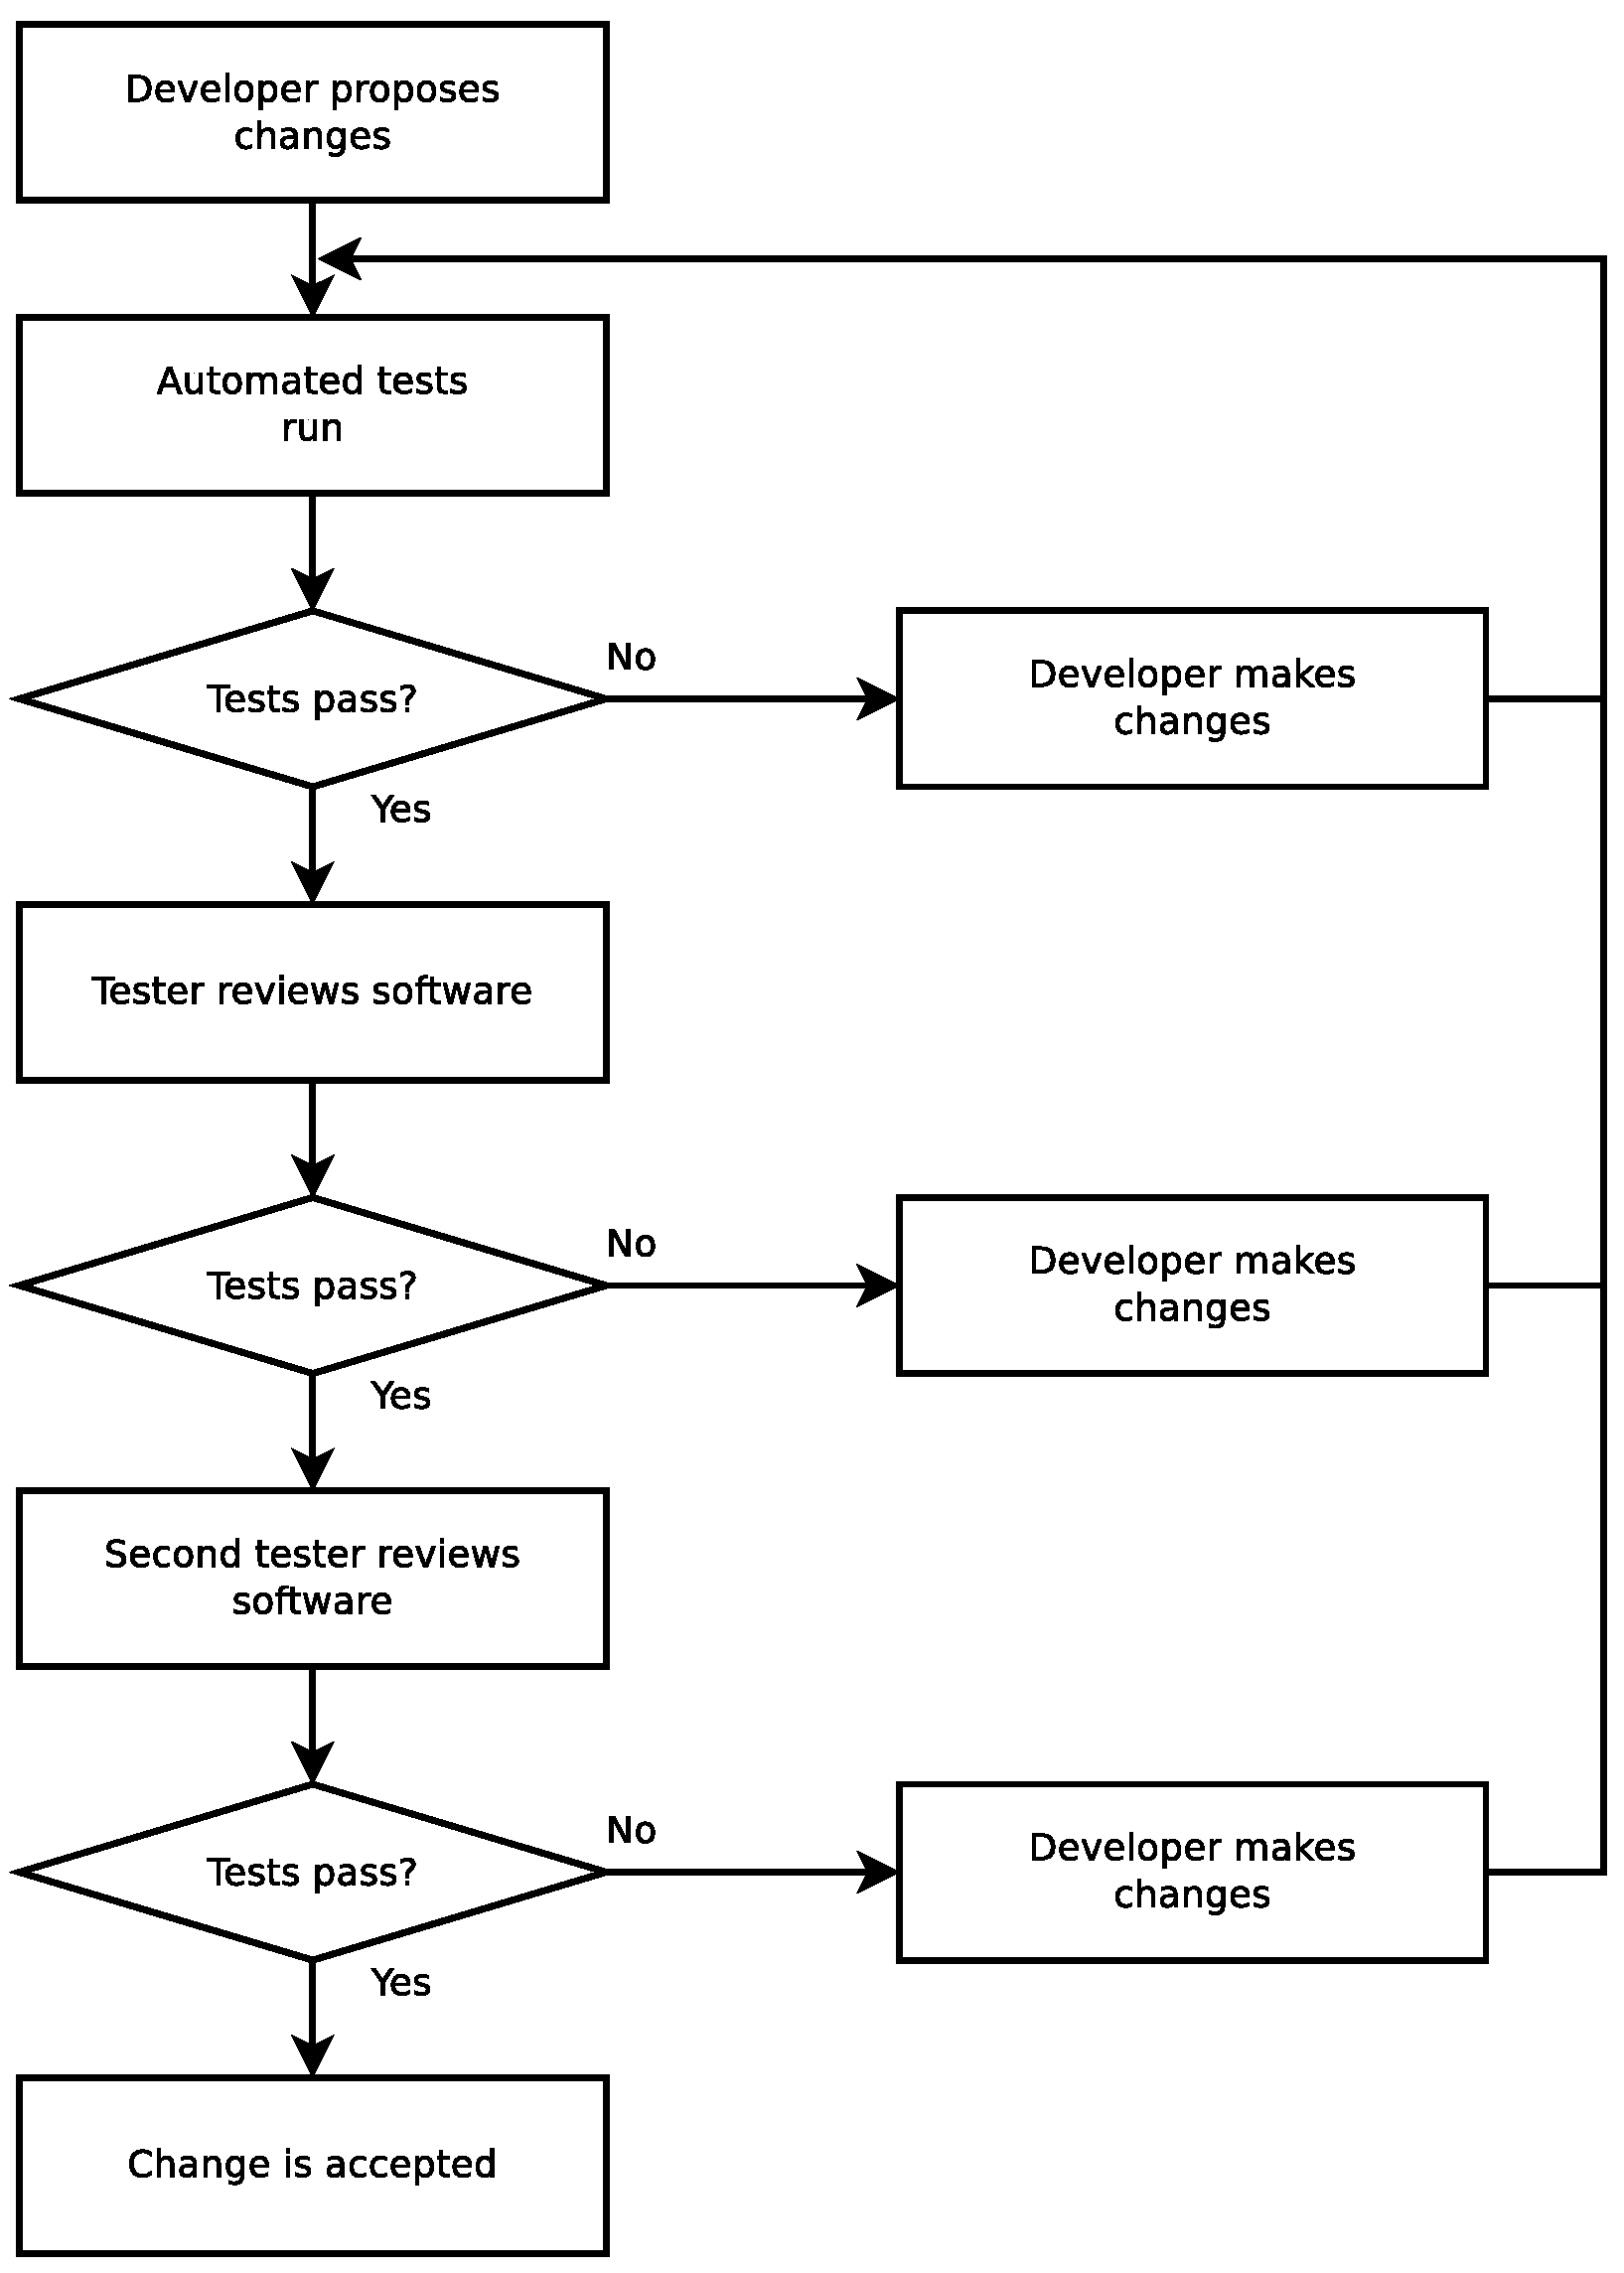
\includegraphics[height=10cm]{code_review_process.eps}
    \caption{This flowchart gives and example of a code review process that may be used in a collaborative project.}
    \label{Code_Review_Process}
\end{figure}

Code reviews  are the process of determining if a proposed change should be added to the code base.
Typically this occurs after a developer has finished working on a feature or bug fix.

The depth of the review process depends on the size and purpose of the project.
The developer proposing the changes should provide instructions on how to test if the changes are successful and why they are necessary.

The reviewer must ensure that the code is of an acceptable quality (coding styles, guidelines, etc. have been followed).
This should also include if the commit history is sensible and the relevant documentation (including release notes) has been updated.
CI tools can be used to perform some of these checks automatically.

Larger or more critical projects may opt to have multiple review stages, in which additional reviewers will perform the same duties as the previous reviewer.
Having multiple reviewers for the same piece of work may seem inefficient, but will increase the chance of potential issues being found before they are added to the code base.

Tools for code reviews are often built into hosted SCM services.
For example, GitHub Pull Requests allow code changes to be viewed and commented on.

\section{Architecture}
\label{Architecture}

A well designed software package would separate its functionality into a set of individual "modules" based on common feature areas.
A module may refer to a package, library or software plugin.

Care should be taken when designing these module.
Each module should perform a very specific task (e.g. minimization) and should only contain the relevant functionality.
Code within a module should be closely related, reducing the need to import unnecessary functionality.
It is possible to test each module in isolation using automated testing (i.e. unit testing), reducing the risk of bugs being introduced into the code base.

A releted pattern in software development is DRY, or "don't repeat yourself" \cite{Foote_2014}.
This pattern encourages having shared code in a common area so that it can be used in multiple different locations.
Otherwise the code base would have multiple implementations of the same functionality, which can lead to them becoming different over time and as a result introducing bugs.

The code base of your software should be managed using an appropriate build system, which will depend on the choice of programming language(s).
A good choice for C and C++ projects is CMake \cite{CMake}.
This can handle setting up library paths and build tools automatically, allowing developers on any platform to build the software locally.
C++ projects can also benefit from use of a dependency manager such as Conan \cite{Conan}.
There are build systems that combine a dependency manager into the build system.
For Python based projects Python's setuptools is typically sufficient, for specific cases (e.g. complex package dependencies) Conda may be used as an alternative.

It can be desirable to allow users to write scripts to further extend the functionality of the software.
Ideally any scripting made available to users should use the Python language.
Python is becoming the standard language for data science and as such has a wide range of libraries, documentation and resources available for it.

If the application requires a graphical user interface (GUI) then a good choice of library is Qt \cite{Qt}.
Qt is an application framework commonly used by many open source and commercial software packages.
It allows easy development of cross platform GUIs in a variety of languages (e.g. C++ and Python).
Another increasingly popular option is to provide a web based interface.

\section{Data Formats and Interoperability}
\label{Data Formats and Interoperability}

It is important to use an open and standardised data format, in order to allow users to easily create suitable input files for the software.
A good data format will have open source definitions and documentation, making it easy to understand and to implement file loaders for the software.
It is likely that a library will already exist for loading standardised file formats and should be used whenever possible.
Any implementation of a standardised data format needs to either follow the standard.
The data format should only diverge from the standard if it is absolutely necessary.
If the divergence from the standard is required and has a clear benefit, then these changes should be suggested to be added to the standard.

In the neutron science community NeXus \cite{K_nnecke_2015} has become the default format.
NeXus aims to standardise the way data is represented by different facilities and software by defining a structure on top of the HDF5 file format \cite{HDF5}.
NeXus is a self describing file format where classes can be used to make it easy to understand the data, with no prior knowledge.
Useful metadata (such as instrument configurations and data processing history) is trivial to store in NeXus.

Proprietary file formats should be avoided at all costs.
While there is sometimes an argument for software specific intermediate formats, they should remain intermediate and NeXus should be the preferred interchange format.

Applications may store relevant information (e.g. window layout for a graphical tool) using the facilities provided by the application framework (e.g. \texttt{QSettings} for Qt).

Additional configuration or process setup information should be stored in an easily accessible location.
This data may include version numbers, parameters and filenames.
This configuration should ideally be in a human readable plain text format, assuming it's data volume does not negate readability or performance.
Popular formats for this purpose include INI, YAML, JSON, TOML and XML, all of which have several library options for common languages and store data as plain text.
Under no circumstances should custom formats be used for configuration files, because there are already a number of well defined data formats for this purpose.

It is vital for the results from scientific software to be reproducible.
However, sometimes there is a need to recreate the results from data treatment, in this case it becomes valuable to be able to replay the series of operations.
Data storage is a concern for most facilities and being able to reproduce data can be beneficial.
An increasingly popular method is to store the unprocessed data and instructions on how to process the data.
This has the advantage of allowing for multiple sets of instructions with a negligible increase in storage space.
This means recording a history of each atomic action the software performs along with any relevant numbers/inputs.

It is essential to be able to extract the exact conditions of the software (i.e. the version number of the software, versions of plugins/dependencies).
Process lists in Savu \cite{Wadeson_2016} are a good example of such operation reporting.
These store the job configuration in a NeXus file and encode the same information in the final results.
This allows the processing history to remain with the processed data and allows the result dataset to be used as input for a future job.
Savu also provides tooling to allow a user to export a list of citations from their result data and is generated from the process list.

\section{Project Management}
\label{Project Management}

Large pieces of software will require some form of management, to ensure that the team are working effectively.
This is often referred to as a governance model.
A governance model will provide a constructive mechanism for deciding the direction of the project and for ensuring it progresses.
This is typically achieved by using project management, which defines a set of guidelines (TODO: cite PFQ https://www.apm.org.uk/book-shop/apm-project-fundamentals-qualification-study-guide/) that will help the project be successful.
Each project will typically have a sponsor(s) who are ultimately responsible for the project, but will not be involved in its running.

The larger the team the more important good project management becomes.
Sections \ref{rman, se} and \ref{lc} will discuss the aspects of project management that would benefit projects of any size.
Then section \ref{PM big} will contain advice for larger teams, but may still be useful to smaller teams.

\subsection{Resource Management}
\label{rman}

Resource management can refer to physical equipment, such as computers.
However, in this context it will be used to refer to individuals who are available to work on the project.
The amount of resource available to a project will probably change over time and it is therefore important to plan how best to utilise each resource.
When selecting a resource for a given task it is important to consider their skills/knowledge, the time required to complete the task and the deadline for the task.
If the deadline and time required are similar then it is better to choose a resource who has the relevant skills and experience.
However, the draw back of always choosing the same resource to do similar tasks is that they will become a single point of failure.
If that resource were to leave the team then no-one else would have any knowledge of that part of the project.
Therefore, it is advisable to use tasks as an opportunity to train less experienced/skilled resources when there is sufficient time between the deadline and the expected duration of the task.

\subsection{Stakeholder Engagement}
\label{se}

Stakeholders is a general term used to describe people who have some interest in your project (e.g. customers, team members and sponsors).
It is up to the individual project to decide what communication method is suitable.

The customers are vital sub-group of stakeholders.
An effective way of keeping them engaged is imperative to the success of the project.
One method is to have a committee (this may be called an advisory committee, in the Mantid project they call it the scientific steering committee).
This group will be comprised of the senior project team (i.e. the project manager and any sub-team leaders for a larger project) and a customer from each of the main user communities.
This committee would discuss the progression of tasks and what tasks should be next (priorities).

\subsection{Software Life Cycle}
\label{lc}

The software should follow the basic notion of a release cycle. More details about the practicalities of a release cycle are discussed in section \ref{Releases}.

A release is a version of the software that has been tested and the development team is confident that it is ready to be used.
Having periodic releases can reassure users that the project is still supported.
It is advisable to follow semantic versioning \cite{Semantic_Versioning} (major.minor.patch, e.g. 3.1.0) for clear naming of the releases.
Prior to a release there will be a "code freeze", where no new functionality will be submitted to the code base.
In preparation for a release developers should test the software works as expected with no obvious bugs.
The next stage is "beta testing", where a select group of users are chosen and they test the software and report any bugs.
Once all of the identified bugs are fixed it is then released with more confidence that it is ready for general use.

It is advisable to then spend some time working on maintenance tasks, these are improvements to the maintainability of the code rather than any new user facing functionality.
Examples of such tasks include: moving to a new compiler version, applying fixes for compiler or linter warnings and code reorganisation/refactoring.

\subsection{Project Management Board and Advisory Committees}
\label{PM big}

It is often beneficial to set up a project management board, who discuss the high level strategy and running of the project.
These will meet fairly irregularly (a few times a year), but would involve the senior team members of the project and key stakeholders (including the sponsor).
This provides an opportunity to discuss possible risks or opportunities and the long term plans for the project.

For larger projects it maybe beneficial to have a technical advisory committee.
This will usually comprise of the technical leads for the project.
Their role is to make decisions on the computational aspects of the project.
For example, which version of a programming language to use and the operating systems that the software will support.
Another role fulfilled by this committee is to decide significant changes to the code base.
This could happen if there is a new method (e.g. standard library algorithms in C++) that can be used throughout the code base to improve performance and/or stability.
A representative from the technical advisory committee will report their decisions to the project management board, who will distribute the information down to the rest of the team.

\section{Licensing}
\label{Licensing}

All pieces of software require a license.
An open source license is advisable from both a user and development perspective, details of available licenses are available online \cite{OSI_Licenses}.
The users will be able to download and use the software free of charge, removing a potential barrier in the uptake of the software.
The advantage of an open source license is that it allows anyone to contribute to the code base (but must not bypass any review process) and radically improves the available pool of developers.
Furthermore, in research/academic communities open source software is becoming increasingly compulsory in order to prevent the loss of valuable source code.

\section{Packaging and Distribution}
\label{Packaging and Distribution}

\subsection{Releases}
\label{Releases}

\begin{figure}
    \centering
    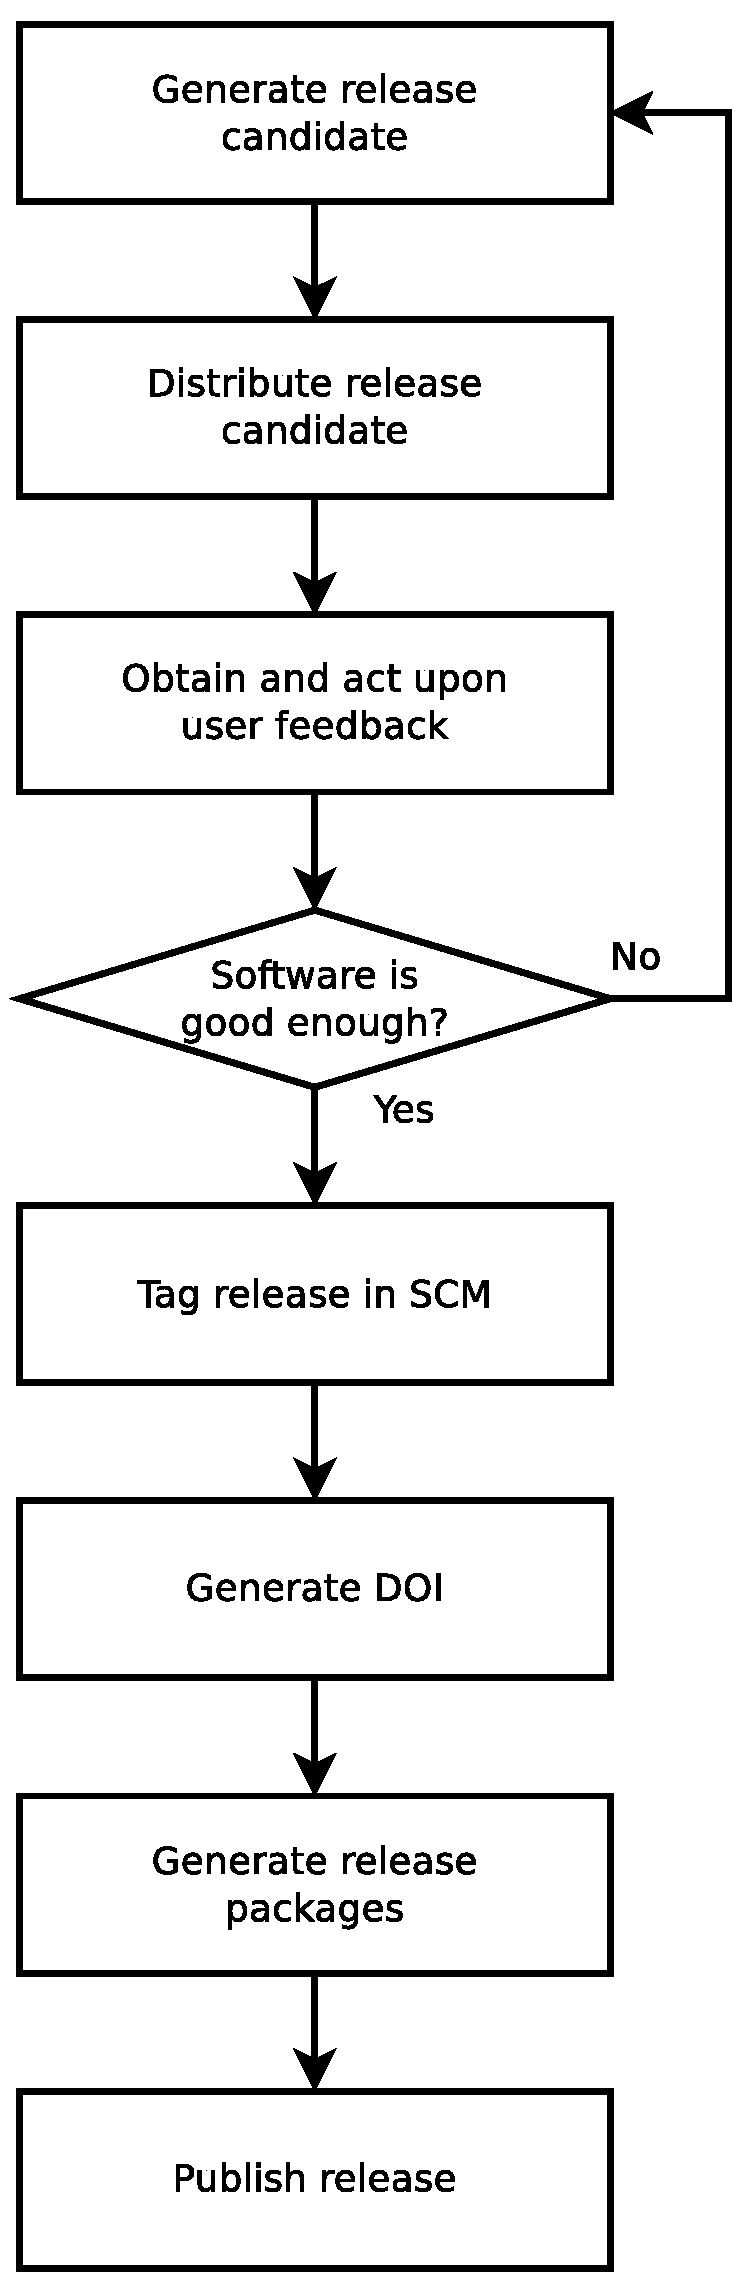
\includegraphics[height=10cm]{release_workflow.eps}
    \caption{This flowchart describes the release workflow for a piece of software.}
    \label{Release_Flowchart}
\end{figure}

A good release process depends greatly on the nature of the software project.
A large framework used by multiple different scientific techniques at different facilities (such as the Mantid project \cite{Manitd}) requires an involved release process to ensure the software is suitable for use by all intended audiences.
This section will assume that a significant proportion of users are not consulted with during the development process.

A release candidate is often used for user testing and for identifying potential issues prior to the main release.
There can be any number of release candidates and they should be generated in exactly the same manner as a release (the only difference being the version number).
Release candidates are intended for "power users" who are happy to test the software for the benefit of the wider community (for example, at a scientist who is responsible for an instrument and its user programme, and who wants to ensure your software works before providing it to their visiting users).

The length of the beta period is determined by the release cycle and the estimated number of users.
There is no generic rule for this, but it is recommended that all (or as close to as possible) use cases of the software have been tested by specialist users.

To ensure users approach the new version with realistic expectations it is essential to provide sufficiently detailed release notes with every version of the software (including release, beta and release candidates).
These should summarise the changes made to the software since the last release, highlighting new features to incentives users to upgrade.

It is essential that all changes that may break existing workflows are listed.
This will reduce the risk of users attempting to use workflows that are no longer compatible with the latest version.

Any fixes for safety or security reasons must be clearly documented in the release notes.

It is recommended to tag and sign the release in the SCM system. In the case of Git this involves creating a tag from the code that was used to generate the release package and signing it with either a project or maintainers PGP (Pretty Good Privacy) key.
This is not an essential step, but is good practice to allow verification of historic releases.

It is also recommended to generate a Digital Object Identifier (DOI) for each release.
This allows the software to be easily cited in publications and makes it clear which version of the software was used to generate the results in a publication.
Another method is to use a publication that provides the idea of the software.

\subsection{Packaging}
\label{Packaging}

To ensure user satisfaction easy software setup is essential.
Exactly what this involves varies depending on the nature of your project, as such this section will not go into great detail about specific options, but rather the requirements of an installer and process of choosing an appropriate installation method for your software.

The first requirement is for the package to give users a working copy of your software.
They should not have to care about any implementation specifics or having to install additional dependencies to make your software run.

Once installed, the software should not conflict with any other software a user may have installed on their machine.
A common example of this is when applications depend on the same libraries, such as HDF5.

It is recommended to sign binaries, this allows a user to verify that the copy of the software they have is in fact the version they believe it is and that it has not been modified.
Some operating systems may also impose restrictions on running unsigned binaries.
How binary signing is done depends on the packaging method and target operating system, it is worth researching this for your specific case.

As the technology becomes more popular it is worth looking into cross platform container based means of distribution (for example, Docker \cite{Docker}, Singularity \cite{Kurtzer_2017} and other container based systems).
This allows the distribution of software in an already configured and working state being safe in the knowledge it will function in the same way on the user's computer.
Different containerization systems have their own caveats and there is no "one size fits all" solution.
For example, Singularity is better at packaging GUI software than Docker, however Docker images are likely to more universally usable due to Docker's popularity.

\subsection{Cross platform}
\label{Cross platform}

Unless your software specifically targets high performance computing systems such as clusters or distributed compute platforms then no assumption can realistically be made about how, and specifically on what platform, a user will expect to run your software.
For this reason it is highly desirable (or even essential) that your software is designed to run on multiple operating systems and architectures.
Thanks to modern development tools, libraries and build systems this is not a complex task.
By using cross platform libraries you also allow your software to be easily adopted by users that use an operating system or environment different to your own.

If officially supporting multiple platforms then it is beneficial to encourage a spread of different platforms and operating systems across your development team.
Doing so ensures that there are always multiple people capable of addressing platform specific issues when they arise.

It is recommended to limit the versions of particular operating systems you support.
Typically you should stop supporting an OS version when the publisher stops supporting it.

Cloud computing is becoming an increasingly common method for delivering software to users. 
Instead of the user providing the computing hardware, an interface layer (e.g. web interface, command line) is provided to a dedicated computing infrastructure. 
One of the main advantages of cloud infrastructure is that the specifications of the operating system and hardware are known by the developer.
This makes it easier to recreate platform specific bugs and if cloud infrastructure is used exclusively it could remove the need for cross platform development.
It is also possible to create a setup where the data is easily accessible from the cloud infrastructure. 
This removes the need for data transfer and storage bottlenecks, which will become increasingly important as data volumes grow.
However, a disadvantage of cloud infrastructure is that it creates an additional dependency.
If the cloud infrastructure is not maintained correctly than the software will become unusable within the cloud service.
The European Open Science Cloud \cite{EOSC} is one example of a project dedicated to this software delivery method.

\subsection{Dependency Management}
\label{Dependency Management}

Dependency management handles obtaining and configuring any library dependencies your software has at build/configure time.
This serves two functions: to make the build environment easy to set up and to make builds reproducible.
Dependency managers do this by collecting requirements for your software based on a specification file provided by the developer.
In the case where a package manager is available (for example Conda \cite{Conda}, PyPI \cite{PyPI} or Conan \cite{Conan}) this may just be a package name and version number.
For more general purpose tools it may involve instructions on how the dependency should be retrieved and configured (for example CMake's ExternalProject \cite{CMake_ExternalProject}).

One of the benefits of dependency management is the ability to pin dependency versions to known working versions.
This ensures that moving to new development or runtime environments will not cause incompatibilities between your software and software it depends on.
It is however important to keep dependencies up to date to ensure known bugs are not included in your software.
The task of updating dependency versions and fixing any issues that arise is a good candidate for a maintenance task (see section \ref{Project Management}).

\section{Support and Documentation}
\label{Support and Documentation}

Good documentation will prevent the developers having to spend time explaining how to use and develop the software to users.
The hallmarks of good documentation are that it is easily available, concise and written in a way that is accessible to the target audience.

The simplest and most common form is online documentation, for example Read the Docs \cite{Read_The_Docs} or a wiki page.
The documentation should have a clear structure and be easy to navigate.
An easy way to achieve this is to have a contents page and to make the pages searchable so users can easily find the relevant information, by having tags that summarise the main themes of each page.
The online documentation should be version controlled so it is possible to revert changes and to follow its evolution.

Projects may benefit from having a landing page introducing the project and directing users to commonly used or important resources.
Examples for this are Hugo \cite{Hugo} and GitHub Pages \cite{GitHub_Pages}.
Hugo is a powerful and fast static website generator.
It supports themeing and customisation and works with content defined in Markdown.
A free hosting service provided by GitHub Pages, this allows you to commit your website content to a specific branch and have it served by GitHub.
The large benefit here is avoiding the cost and time of maintaining the infrastructure required to host the project's website.

An increasingly popular method of documentation is the video tutorial.
These are extremely useful to users as it allows them to see how the software is used.
For example, video tutorials of intricate GUIs may be beneficial as the user gets to see a complete workflow and there is less chance of steps being undocumented.
However video tutorials can be costly to create and keep up-to-date with software changes.

Face to face communication is often the most efficient and effective way to understand a user's question/comment.
This allows for a conversation to occur with more probing questions to improve the developer's understanding and to overcome any unfamiliar terminology.
As a result it is important to have some local support, where developers are preferably in close proximity to their users.
Face to face contact also has the benefit of increasing the user experience and users are more likely to report problems/bugs to the development team if they can easily speak to them.

A key activity for any piece of software is user support.
Unlike documentation this is an interactive link between developers and users.
As a minimum email support should be provided and users made aware of it.
The emails should be checked regularly and initial responses should be within a day or two.
The initial response may be to ask for more details, to arrange a meeting or to say that it is being worked on.
Providing effective user support will give users more confidence in the software.

The documentation discussed so far has focused on the users.
It is also valuable to have developer documentation.
This documentation should contain information on the standards used in the code and how to set up a development environment, appropriate tutorials and relevant reference material.

\section{SINE2020}
\label{SINE2020}

This section describes guidelines specific to the development of data treatment software for the neutron and muon communities.
The specific guidelines in this section may not be suitable for other communities.

These specific guidelines were developed as part of the data treatment work package (WP 10) of Science and Innovation with Neutrons in Europe in 2020 (SINE2020).
This was a 4-year project between 18 partner institutions spread across 12 different countries.
The first deliverable (D10.1) was to write the standards and guidelines for software developed as part of SINE2020, with the aim of developing collaborative and interoperable software.

The report \cite{sine2020_wp10_d10_report} contains the standards and guidelines that were used for WP10 of SINE2020.
This report contains statistics and information about neutron and muon data treatment software including tables identifying commonality.
The guidelines are designed to be specific enough to ensure commonality between different pieces of software, but sufficiently abstract to not be restrictive.
The main guidelines are presented below with references to the relevant section of this paper for further reading.

\begin{itemize}
      \item Use an Open Source license, such as GPL.
      \item Support multiple operation systems.
      \item Design software to be modular.
      \item Use the programming languages C++ and/or Python.
      \item Where the software uses a GUI, use Qt.
      \item Support loading of NeXus/HDF5 data formats where such exists.
      \item Use Git for version control of source code including for user and developer documentation.
      \item Use a issue/ticketing system; such as Github issues.
      \item Use a tool for continuous integration and automated testing; such as Travis-CI and Jenkins
      \item Follow a coding standard and use tools that enforces this; such as Pylint (Python) and ClangFormat (C++).
\end{itemize}
\begin{sidewaystable}[]
 \begin{tabular}{llllll}
 Software                        & BornAgain \cite{}  & Mantid \cite{} &McStats \cite{}  &MuhRec \cite{} & SasView \cite{} \\
 Age of project (years)          & 9 & 11 & 21 & 10 & 15 \\
 Number of developers (full time)& 3 & 20 & 5 & 2 & 2-20 \\
 Developer locations             & 1 & >4 & TODO & 1 & TODO \\
 License                         & GPLv3 & GPLv3 & GPLv2 & GPLv3 & BSD \\
 Governance model                & None & PMB \& AC  & None & AC & PMB \\
 Release cycles (per year)       & a few & 3 & 1 & 1 & 1\\
 User documentation              & Tutorials. Examples. & Manual. Tutorials. & Manual. & Manual. & Manual. Tutorials.
 \end{tabular}
 \caption{An updated summary of how guidelines were applied to the different software projects from SINE200 \cite{} (TODO: ref paper). The number of guidelines implemented increases with the size
and scope of the project. PMB = Project Management Board. AC = Advisory Committee}
\label{summaryTable}
\end{sidewaystable}

The statistics of how guidelines could be applied to software projects are presented in table \ref{summaryTable}.
Some of the projects have a large numbers of developers and/or based at multiple locations.
As a result the management overheads (e.g. project management boards) are greater to ensure a uniform standard across the project.
The projects with less developers tend to have less management overheads as it is easier to make decisions across the whole team.
This is a good example of how guidelines should be adapted to match the needs of the project.

\section{Conclusion}
\label{Conclusion}

Scientific software is becoming an increasingly valuable tool for research.
However, the cost of implementing such software can be high and as a result it is beneficial to write sustainable software.
The best way to achieve sustainable software is to implement guidelines.
This paper has outlined a series of guidelines for scientific software development.
The guidelines have covered a range of topics from coding standards to management of the software and customers.

Fundamentally guidelines allow for scientific software to be developed and maintained easily by a distributed team, while providing support to users.
There is an initial cost in deciding the guidelines and they should be chosen based on the requirements of the project.
To ensure that there is a balance between new functionality and maintenance it is important to manage the customers and to have a governance model.
To ensure a happy user base it is important to have up to date documentation and to have regular releases.
The technologies available to software development are constantly changing and for long term projects it may be necessary to update the guidelines to utilise these improvements.
Good guidelines ensure a uniform code quality, a structured developer team and create a positive user experience.
These factors will help create a stable, maintainable piece of software and increase the likelihood of the software's user base flourishing.

\section{Acknowledgements}
\label{Acknowledgements}

Thanks to Ed Beard for initial proofreading.

Thanks to Robert Applin and Dimitar Tasev for additional proofreading.

This work was funded by the Horizon 2020 Framework Programme of the European Union.
Project number 654000.

%%%%%%%%%%% The bibliography starts:

%%%%%%%%%%%%%%%%%%%%%%%%%%%%%%%%%%%%%%%%%%%%%%%%%%%%%%%%%%%%%
%%                  The Bibliography                       %%
%%                                                         %%
%%  ios1.bst will be used to                               %%
%%  create a .BBL file for submission.                     %%
%%                                                         %%
%%                                                         %%
%%  Note that the displayed Bibliography will not          %%
%%  necessarily be rendered by Latex exactly as specified  %%
%%  in the online Instructions for Authors.                %%
%%                                                         %%
%%%%%%%%%%%%%%%%%%%%%%%%%%%%%%%%%%%%%%%%%%%%%%%%%%%%%%%%%%%%%

\nocite{*}
\bibliographystyle{ios1}
\bibliography{bibliography}

\end{document}
